%% USPSC-Introducao.tex

% ----------------------------------------------------------
% Introdução (exemplo de capítulo sem numeração, mas presente no Sumário)
% ----------------------------------------------------------
\chapter[Introduction]{Introduction}
\label{Introduction}

In 1985, the first interaction between medicine and robotics occurred with the \textit{PUMA} manipulator, which was used for brain biopsies — a procedure that removes a small piece of brain tissue for analysis. Surgical interventions further expanded with the introduction of the \textit{da Vinci} robot, enabling tasks to be performed with precision and strength beyond human capability, and allowing surgeons to execute procedures that would be very difficult without robotic assistance \cite{morrell2021history}.

At the end of the 20th century, there was a fundamental transformation in the methods used to perform surgical procedures. For many interventions, the invasive nature has been considerably reduced, bringing superior results such as better survival rates, lower incidence of complications, and faster recovery in terms of functional health and quality of life. This emphasis on less invasive approaches, also known as minimally invasive surgery (MIS), has been gaining momentum and has been the subject of intensive research and development of new surgical techniques in recent years \cite{minimal}.

% spine robots intro? types of robots? collaborative robots?

Neuromate was introduced in the late 1990s as one of the first robotic systems dedicated to intracranial electrode implantation, providing automated and accurate positioning for neurosurgical procedures. These procedures include SEEG (stereoelectroencephalography), which is primarily used for the diagnosis and treatment of epilepsy by enabling the precise placement of electrodes to identify seizure foci deep within the brain. Other applications are DBS (deep brain stimulation) for movement disorders such as Parkinson's disease, and brain biopsies for diagnostic purposes.

ROSA followed as a next-generation platform, integrating advanced planning and navigation tools. The benefits provided by the robotic systems are essential in epilepsy surgery, where the correct localization and targeting of epileptogenic zones can significantly improve patient outcomes.
This work aims to develop a robotic system for intracranial electrode placement in SEEG surgeries for epilepsy treatment. For context, it is important to review the characteristics of epilepsy (Section \ref{sec:epi}), the types of seizures and their effects on patients, and the current treatment approaches (Section \ref{sec:methods}).

\section{Epilepsy}\label{sec:epi}

% @gui one for what is epilepsy
%...
\textit{Epilepsy} is a chronic brain disease characterized by a long-lasting predisposition to generate seizures, not caused by any immediate insult to the central nervous system, and by the neurobiological, cognitive, psychological, and social consequences of recurrent seizures \cite{beghi2020epidemiology}. This is the most common neurological disease worldwide, affecting different social classes, races, ages, and geographic locations \cite{ngugi2010estimation}.

% what is epilepsy seizures
The definition of \textit{epileptic seizures} is: repeated and transient episodes that manifest themselves through patterned behaviors, mirroring the underlying neural processes associated with the condition \cite{fisher2005epileptic}. Although all people with epilepsy experience seizures, not all individuals with seizures have epilepsy. Epileptic seizures can also occur after an acute injury to the central nervous system (CNS) of structural, systemic, toxic, or metabolic origin. These events are considered acute manifestations of the insult and may not occur when the underlying cause has been removed or the acute phase has passed \cite{beghi2010recommendation}.

% types of epilepsy seizures
Epileptic seizures are categorized according to three main characteristics: origin in the brain, state of consciousness during the seizure, and level of body movement. Seizures can be classified as focal or generalized based on the first characteristic. The second characteristic considers whether consciousness is intact or impaired during the seizure, while the third characteristic refers to body movement, which may present motor or non-motor reactions \cite{beghi2020epidemiology}.

Motor seizures encompass a variety of distinct manifestations. Atonic crises are characterized by a sudden and temporary loss of muscle tone, resulting in a sudden fall of the individual. On the other hand, tonic crises involve a sudden and prolonged increase in muscle tone, leading to intense stiffness. Clonic seizures are marked by rhythmic and repetitive muscle contractions, which can affect different parts of the body, while myoclonic seizures are characterized by rapid and sudden muscle contractions that can involve a specific muscle group or the entire body. Epileptic spasms, automatisms, and hyperkinetic seizures are also categorized \cite{sarmast2020current}.

On the other hand, non-motor crises can present different forms of manifestation. They can be autonomic, involving dysfunctions in the autonomic nervous system, such as changes in blood pressure or heart rate. In addition, there may be crises of behavioral arrest, during which the individual may appear paralyzed or unable to perform voluntary movements. Cognitive crises affect cognitive function and may include memory lapses or mental confusion. Emotional crises are related to changes in the emotional state, such as feelings of fear, anxiety, or euphoria. Finally, sensory crises affect the senses and can cause abnormal sensations, such as visual or auditory hallucinations \cite{sarmast2020current}.

\section{Treatment methods} \label{sec:methods}

% @gui one for what are the treatments
%...
Among patients with epilepsy, approximately 30\% experience drug-resistant seizures, representing a significant portion of the global population, estimated at 70 million people. In such cases, resective surgery appears as a viable therapeutic option. This procedure is considered in patients with disabling focal epilepsy who are unresponsive to drug treatment and whose seizures originate in a specific region of the brain that can be removed with minimal risk of neurological or cognitive dysfunction \cite{miller2013surgical}. Resective surgery offers the possibility of significantly improving the quality of life of these patients, providing adequate control of seizures and reducing dependence on high-cost and potentially harmful antiepileptic medications.

Correctly locating the focus of seizures is a crucial aspect in preparing for resective surgery in patients with epilepsy \cite{miller2013surgical}. Localization methods are applied to accurately determine the focal region, aiming to minimize the invasiveness of the surgery while seeking complete removal of the area of focus to cease seizures. Accuracy in locating the focus has a significant impact on the effectiveness of the surgical procedure, as it can help avoid undesirable consequences associated with the resection of unaffected areas.

This is especially important, as the removal of critical areas of the brain can result in functional deficits, such as impairment of speech, memory, motor coordination, among other functions, depending on the location of the focus. Therefore, ensuring accurate location of the focus is essential to guarantee good surgical results and minimize potential adverse effects.

\subsection{Non-invasive video-EEG}

% @gui EEG
%...
Before considering invasive procedures, a non-invasive analysis is typically performed to identify potential areas of seizure foci and to guide further investigation. Scalp EEG is the primary non-invasive technique used for this purpose. Electrodes are placed on the patient's scalp using a cap or similar device, enabling monitoring during interictal (between seizures), ictal (during seizures), and post-ictal (after seizures) periods. This superficial electrode arrangement measures electrical potentials generated by neuronal activity near the skull. Standard systems use 32, 64, or 96 electrodes distributed across the scalp, with higher-density arrays (up to 256 channels) available for more detailed studies \cite{Sun2023}. Scalp EEG is essential for initial diagnosis and localization of seizure activity, providing critical information before invasive methods are considered \cite{miller2013surgical}.

\subsection{Invasive EEG: Subdural EEG (SDE) and Stereoencephalography (SEEG)}

%@gui subdural EEG
%...
Subdural EEG (SDE), also known as electrocorticography (ECoG), was developed to provide more precise measurement of brain activity than scalp EEG. In SDE, an electrode array is placed directly on the surface of the cortex after a portion of the skull is removed, as illustrated in Figure \ref{fig:eeg-ecog-seeg}. This direct contact enables the acquisition of signals with higher fidelity and less noise compared to scalp EEG \cite{lesser2010subdural}. The electrodes typically remain in place for several days to record both ictal and interictal activity. However, SDE is highly invasive, requiring two craniotomies — one for electrode placement and another for removal — and carries a significant risk of postoperative infection, often related to surgical contamination. These drawbacks have motivated the development of alternative methods, such as SEEG, which aim to reduce invasiveness and associated complications \cite{jehi2021comparative}.

% @gui SEEG
%...
In France, in the 1950s, Jean Tailarach and Jean Bancaud developed a method that aims to monitor deep parts of the cortex through the insertion of deep electrodes, seeking to replace the SDE \cite{mazoyer2008memoriam}. This method was called Stereoelectroencephalography (SEEG) and today it is one of the most adopted invasive methods for locating the focal zone of seizures. SEEG does not present many of the problems presented by SDE. In this method, cylindrical electrodes (more like small wires) are introduced through small holes in the skull, without the need for craniotomy. SEEG has lower rates of infection, hemorrhage, neurological deficits, and morbidity compared to SDE, in addition to being a faster procedure, allowing the analysis of deeper brain tissues and having shown greater effectiveness in localizing and controlling seizures after surgical treatment \cite{fiani2021stereoelectroencephalography}. Figure \ref{fig:eeg-ecog-seeg} illustrates the positioning of electrodes in scalp EEG, Subdural EEG (electrocorticography), and SEEG.

% fig scalp eeg, ecog and seeg
\begin{figure}
     \centering
     \includegraphics[width=0.99\textwidth]{USPSC-img/eeg-ecog-seeg.png}
     \caption{Positioning of electrodes in scalp electroencephalography, electrocorticography, and stereoelectroencephalography procedures respectively \cite{shen2020ml} \cite{blausen2014medical} \cite{Jones2018}.}
     \label{fig:eeg-ecog-seeg}
\end{figure}

% Metrics for analyzing the accuracy
%...euclidean distance and etc
Electrodes implanted by SEEG must be precisely placed for proper identification of the epileptogenic zone (EZ) \cite{Jones2018}. Planning prior to surgery is carried out to define the number of electrodes, the position of the entry points, and the target point of each electrode. Metrics are defined for evaluating the effectiveness of SEEG operations, constituting a basis for evaluating different SEEG methods. Entry points are defined as the point at which the electrode initiates contact with the surface of the brain. Target points are defined as the final position of the electrode, usually in a region within the brain. Widely adopted metrics are the Euclidean distance between the planned entry points and the post-surgical entry points, the distance between the planned target points and the post-surgical target points, and the angle between the two vectors formed by the planned and post-surgical entry and target points representing the orientation error.

\section{Stereoelectroencephalography: operation methods} \label{sec:seeg-methods}

% classic methods of SEEG
% Stereotactic Arc...
% Tailarach
%...
SEEG operation techniques began with Tailarach using x-ray images for planning and checking electrode positioning. Since the inception of SEEG, the development of mechanical stereotaxic apparatus that fix the skull and guide electrode placement has been the focus to achieve the best precision during surgery. The first apparatus was called the Tailarach apparatus and featured pins for fixing the skull, support for the x-ray tube, and radiographic film \cite{mazoyer2008memoriam}.Popular devices today date their creation to the same time, such as the Leksell in Sweden.

With the advent of computed tomography, surgeries began to be planned based on slices, allowing a three-dimensional understanding of the areas of investigation. Devices that use the three-dimensionality of tomography images were adapted, adding a support with a diagonal cut in the shape of an N, allowing the calculation of the height of each tomography slice in relation to the device coordinates. This system became known as the \textit{N-Localizer} and is widely used in current neurosurgeries \cite{lozano2009textbook}.

\begin{figure}[h]
   \centering
   \subfigure[]{\includegraphics[width=0.69\textwidth]{USPSC-img/tailarach-frame.jpg}} 
   \subfigure[]{\includegraphics[width=0.29\textwidth]{USPSC-img/tailarach-coordinates.jpeg}} 
   \caption{(a) presents Tailarach's \textit{frame} with x-ray supports and (b) presents an example x-ray image alongside the coordinate system developed by Tailarach \cite{mazoyer2008memoriam}.}
\end{figure}

\subsection{Frame-based surgeries} \label{sec:stereotatics}

The original SEEG technique consisted of introducing parallel electrodes, at least, to an orthogonal sagittal or coronal view using the Cartesian map called Tailarach coordinates \cite{mazoyer2008memoriam}. Subsequently, variations of the technique were explored with the introduction of stereotaxic arcs that can be fixed to devices such as the Leksell or CRW and that allow the introduction of oblique electrodes. Therefore, the assessment of the impact on precision between different techniques for implanting oblique or orthogonal electrodes was studied in \cite{Iordanou2019}. Figure \ref{fig:leksell} presents the Leksell G apparatus and the N-Localizer.

Originally, the calculation of the coordinates of each electrode in relation to the apparatus was carried out manually, using the \textit{N-Localizer} geometry. Software for surgical planning was developed so that the calculation of the coordinates of the entry and target points was automated using image processing methods containing the N-Localizer \cite{dasgupta2022previous}. These software also feature crucial planning tools, such as fusing standard CT images and MRI images.

% fig leksell
\begin{figure}[h]
     \centering
     \includegraphics[width=0.7\textwidth]{USPSC-img/leksell.png}
     \caption{Frame Leksell G without N-Localizer and with N-Localizer respectively \cite{rojas2016eval}.}
     \label{fig:leksell}
\end{figure}

Image fusion allows precise surgical planning by combining preoperative CT and MRI scans to assess vascular structures and functional anatomy near electrode trajectories. During surgery, a stereotactic frame and N-Localizer are attached to the patient's head, followed by an intraoperative CT scan. This scan is fused with the preoperative images, enabling the planning software to identify N-Localizer fiducials and accurately compute coordinates for electrode placement. These coordinates are then inputted into the stereotactic frame or arc, guiding the surgeon in positioning each electrode along the planned trajectory.

%In this regard, Medtronic, with the Stealth Autoguide \cite{medtronic}, developed a system that allows the tool to be fixed, facilitating the drilling of the skull and the fixation of the guide screw.

Surgeries based on stereotactic devices have a broad history of use, but they also have disadvantages in relation to more recent systems, such as robotic systems. Among the disadvantages, the stereotaxic \textit{frames} operation requires the placement of the apparatus at the beginning of the surgery, the performance of a tomography with the N-Localizer, and the fusion of this volume with the CT and MRI images taken (generally days before surgery) used for planning. This process is necessary to calculate the coordinates of each entry point and target in relation to the frame. This process is not necessary with the use of robotic systems in surgeries called \textit{frameless}, in which a stereotaxic apparatus is not used.

\begin{table}[!h]
     \centering
     \caption{Comparison between frame-based and \textit{frameless} procedures for SEEG.}
     \label{tab:frame-vs-frameless}
     \begin{tabular}{p{0.95\linewidth}}
         \toprule
         Surgery based on stereotactic apparatus. \\
         \toprule
         1. CT, MRI and preliminary surgery exams.
        
         2. Orthogonal trajectory planning based on preliminary evidence before surgery.

         3. Start of surgery and fixation of the head in the stereotaxic apparatus (Leksell).
        
         4. Tomography with Leksell and \textit{N-Localizer}

         5. Fusion of CT, MRI and CT images with Leksell to calculate the coordinates of each electrode in relation to the apparatus
        
         6. Using the stereotaxic ruler, drill the skin and skull using a 3 mm drill with an appropriate end point.
        
         7. Fixing the guide screw to the skull
        
         8. Using the guide screw, insert the temporary stylet into the intracranial space to the target point for electrode guidance.
        
         9. Remove the temporary stylet and, through the guide screw, insert the depth electrode into the intracranial space to the predefined destination.
        
         10. Screw the electrode cover onto the guide screw.
        
         11. Repeat steps 6 to 10 for the remaining electrodes. \\
         \bottomrule
          \\
         \toprule
         Robot-assisted surgery \\
         \toprule
         1. CT, MRI and preliminary surgery exams.
        
         2. Planning orthogonal trajectories based on preliminary evidence before surgery using the robot's neuronavigator.

         3. Facial registration using fiducial points of the face
        
         4. Positioning the robot and drilling the skin and skull using a 3 mm drill with an appropriate limit stroke.
        
         5. Fixing the guide screw to the skull
        
         6. Using the guide screw, insert the temporary stylet into the intracranial space to the target point for electrode guidance.
        
         7. Remove the temporary stylet and, through the guide screw, insert the depth electrode into the intracranial space to the predefined destination.
        
         8. Screw the electrode cover onto the guide screw.
        
         9. Repeat steps 4 to 8 for the remaining electrodes. \\
         \bottomrule
     \end{tabular}
\end{table}

The Table \ref{tab:frame-vs-frameless} presents a comparison between the procedures necessary to perform \textit{frame-based} surgery compared to \textit{frameless} surgeries. The greater number of steps during surgery increases the time needed to perform the surgery and may result in loss of accuracy due to non-deterministic procedures and possible human errors.

Performing a CT scan during surgery is time-consuming and ideally should be avoided whenever possible. The frame-based process requires a tomography with the stereotactic device immediately after its placement. While having a CT scanner available in the same operating room would streamline logistics, this setup is rarely feasible, as most hospitals do not have a dedicated CT scanner for each operating room. Although some facilities offer operating rooms equipped with CT scanners, their limited availability and competition with other ongoing surgeries complicate scheduling and scalability. As a result, the typical solution is to transport the sedated patient to a separate CT scanner, which increases surgery time and introduces risks of unwanted movement or disturbance to the apparatus during transport, potentially compromising surgical accuracy.

After the tomography with the device, the fusion of intraoperative CT images generated with the device and preoperative MRI images is also a source of errors. In more detail, image fusion consists of aligning two volumes (the set of slices generated in CT and MRI) so that they both represent the same anatomical region. This is necessary because the volume resulting from the CT scanner depends on factors such as the patient's position and the coordinate system intrinsic to the CT. The alignment of the preoperative MRI with the intraoperative CT, in the case of SEEG surgery, allows the planning performed on the MRI to be accurately transferred to the CT acquired with the stereotaxic apparatus. In this way, the result of the fusion is the planning of the surgery, containing entry and target points in the same reference as the apparatus images, thus allowing the calculation of the coordinates necessary to align the ruler or stereotaxic arc in each trajectory.

However, the alignment of CT images presents an error caused by the method used for alignment. Alignment algorithms can use the intensities of each \textit{pixel} for the best alignment, as well as manually selected fiducial points to minimize the fusion error. Even in the most ideal case, this process is not perfect and will contribute to the final error of each trajectory. In short, fixing the device, transporting it to the CT scanner, and fusion of images are some of the sources of errors during surgeries based on stereotactic devices.

\subsection{Robot-based surgeries}

\begin{figure}
     \centering
     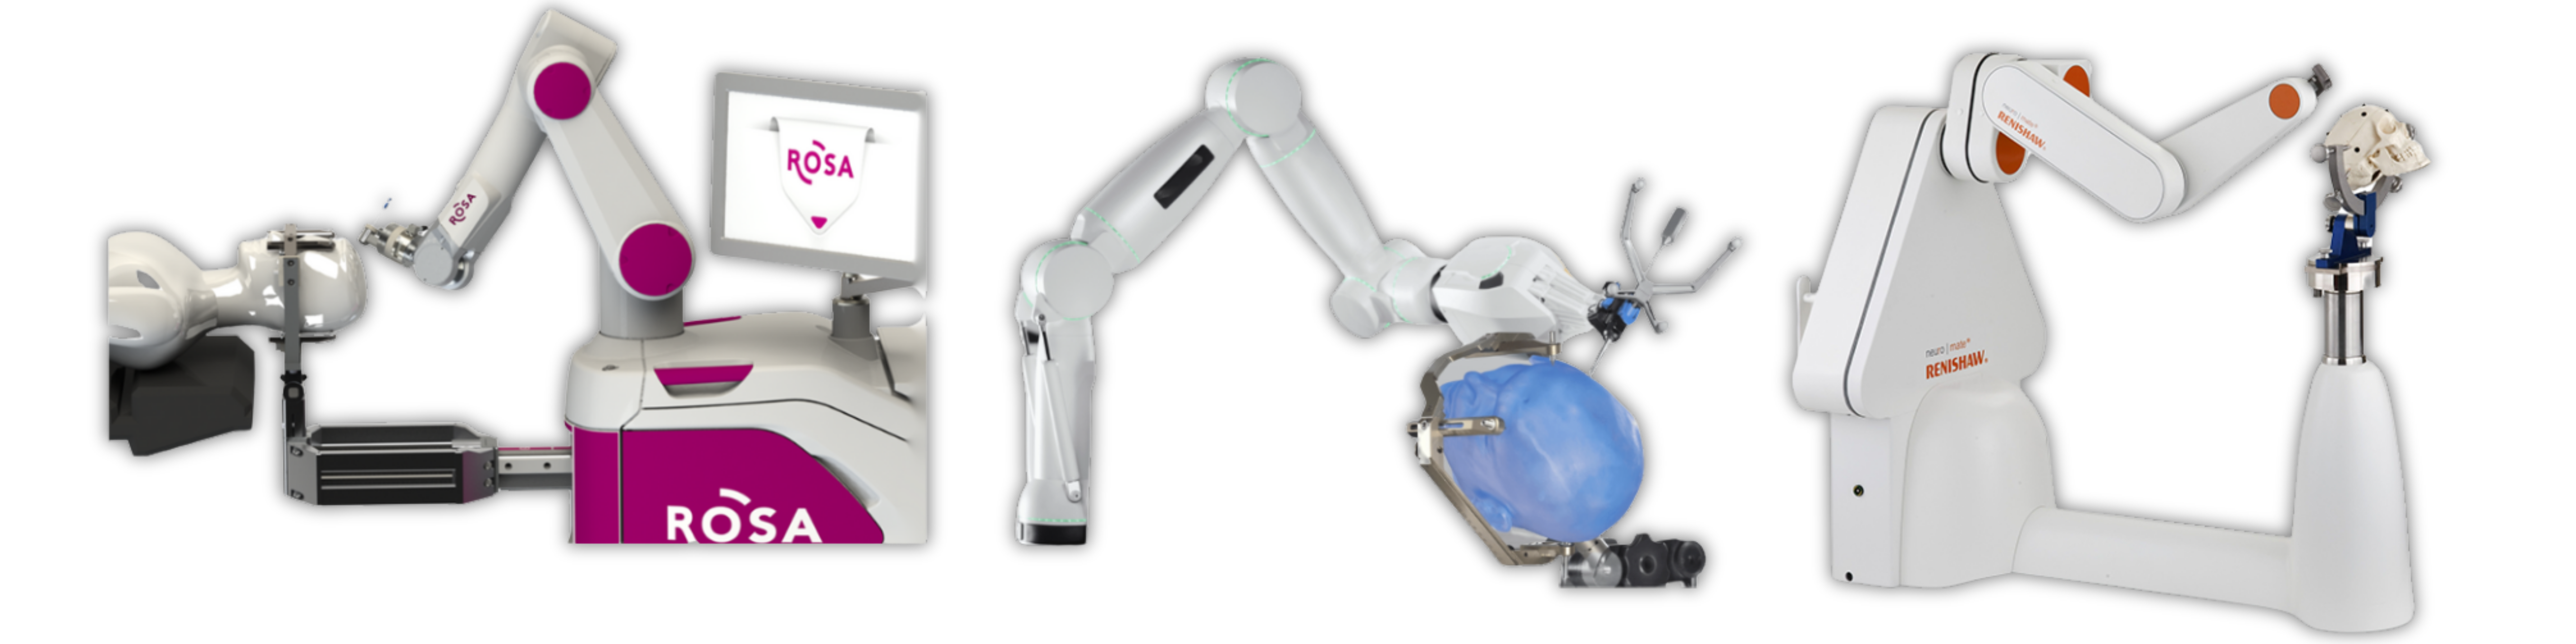
\includegraphics[width=0.99\textwidth]{USPSC-img/robots_enhanced.png}
     \caption{Competing robots capable of performing SEEG surgeries: Zimmer Biomet ROSA ONE Brain, Brainlab Cirq and Renishaw Neuromate respectively.}
     \label{fig:robots}
\end{figure}

Recent advances in the literature highlight the development of \textit{frameless} robotic systems for SEEG surgeries, aiming to improve surgical workflow, precision, and safety \cite{gonzalez2016technique, cardinale2013stereoelectroencephalography}. Renishaw's Neuromate, introduced in 1998, was the first commercially available robot for SEEG neurosurgery \cite{cardinale2013stereoelectroencephalography}. Figure \ref{fig:robots} shows Neuromate, which features a triangular base and supports for skull fixation using Mayfield or Leksell frames. Subsequently, Medtech (acquired by Zimmer Biomet) developed ROSA ONE Brain, and Brainlab introduced Cirq, both capable of performing SEEG procedures. These systems also support other neurosurgical interventions, including brain biopsies and deep brain stimulation (DBS) for conditions such as Parkinson's disease.

% neuromate
Neuromate was the first commercially available robot for neurosurgery, but its adoption faces significant limitations \cite{kajita2015installation}. A major constraint is the requirement for a dedicated operating room, as the system is not designed for mobility between rooms. This complicates hospital logistics and often prevents acquisition due to infrastructure demands. Additionally, Neuromate features only 5 degrees of freedom (DOF), making it an under-actuated system with reduced mobility and positioning capabilities compared to conventional 6-DOF robotic platforms.

% cirq
The Cirq robotic system is used as a neuronavigation tool. A device with reflective spheres is fixed to the robot's flange, similar to that used in common neuronavigators. This device is viewed by an infrared stereo camera and the position of the tool is calculated. Each joint of the robot has only brakes and, therefore, is not actuated, but allows the system to remain static during procedures.

Its adjustment is done semi-automatically, where the surgeon approaches the robot to the desired position and the robot adjusts itself with an actuator fixed to its flange. The neuronavigator is used to operate this system, which has: a camera carriage; a screen carriage; and a robotic manipulator fixed to the operating table. Combined with other devices present in the operating room, these three devices bring difficulties in logistics and in organizing the space in the room compared to systems that have only one carriage.

ROSA ONE Brain, unlike Cirq, for example, is not collaborative. In other words, even though it is designed to perform a task together with the surgeon, ROSA does not feature sensors that are present in collaborative systems, such as measuring joint torque, collision detection, and automatic braking when an emergency is activated. This aspect makes ROSA a conventional robot applied to collaborative tasks, putting doctor and patient safety at risk. Yara, the system proposed in this project, uses collaborative systems, validated worldwide for tasks that involve joint operations with humans, ensuring the surgeon's safety.

ROSA is a conventional industrial robot and does not feature collaborative capabilities, limiting its ability to sense and respond to its environment. This poses potential safety risks for both patients and surgeons. Typically, non-collaborative industrial robots are required to operate at a safe distance from humans according to workplace safety regulations, but surgical robots are not subject to these industrial standards. Current commercial neurosurgical systems do not incorporate collaborative robotics technology. KUKA pioneered the introduction of collaborative robots for medical applications with the KUKA LBR Med, which is certified according to international medical safety standards. Collaborative systems like these enhance safety during robotic manipulation in surgery, offering advantages over existing non-collaborative platforms.

The Stealth AutoGuide by Medtronic \cite{medtronic} is a compact robotic system that attaches directly to the Mayfield head clamp, rather than functioning as a full robotic arm. It assists the surgeon by aligning the trajectory of each electrode during SEEG procedures. The system operates in conjunction with their neuronavigation platform, which is widely used for image-guided surgery. Neuronavigation systems typically employ either optical (stereo camera) or electromagnetic tracking to display instrument positions relative to the patient's anatomy, using preoperative CT or MRI data to guide access to specific brain targets. By integrating with these systems, the small robot arm improves the accuracy of electrode placement, providing precise guidance along planned trajectories.


\section{Introducing Yara}

Yara is a collaborative robotic platform designed for frameless intracranial electrode placement procedures, offering increased precision, reduced surgical time, and lower risk compared to frame-based methods. The system prioritizes surgeon safety and usability, featuring planning software for electrode entry and target points, MRI/CT image fusion, automated patient registration via depth cameras, and collision-free robotic alignment. Additionally, the robot functions as a neuronavigation system, expanding its range of supported neurosurgical procedures like brain tumor removal.

% %%%%%%%%%%%

The \textit{Yara} system is initially targeted for SEEG procedures, with plans to expand its use to brain biopsy and DBS surgeries following successful validation in human cases. SEEG is prioritized due to its less stringent accuracy requirements compared to DBS and biopsy. After completing SEEG validation, further testing will be conducted for DBS and biopsy applications, positioning Yara alongside established systems such as ROSA, Neuromate, and Cirq in terms of supported neurosurgical procedures.